\documentclass[11pt,a4paper]{article}
\usepackage[utf8x]{inputenc}
\usepackage{ucs}
\usepackage[spanish]{babel}
\usepackage[left=2cm,top=4cm,right=2cm,bottom=3cm]{geometry} 
\usepackage{amsmath}
\usepackage{amsfonts}
\usepackage{amssymb}
\usepackage{dcolumn}
\usepackage{float}
\usepackage{graphicx}
\usepackage{ esint }
\usepackage{fancyhdr}
\usepackage{enumerate} 
\pagestyle{fancy}
\usepackage{tocbibind}
\usepackage{setspace}
\usepackage{parskip}
\usepackage[hidelinks]{hyperref}
\usepackage{listings} 
\usepackage[svgnames]{xcolor}

\definecolor{codegreen}{rgb}{0,0.6,0}
\definecolor{codegray}{rgb}{0.5,0.5,0.5}
\definecolor{codepurple}{rgb}{0.58,0,0.82}
\definecolor{backcolour}{rgb}{0.95,0.95,0.92}


\definecolor{dkgreen}{rgb}{0,0.6,0}
\definecolor{gray}{rgb}{0.5,0.5,0.5}
\definecolor{mauve}{rgb}{0.58,0,0.82}


\lstset{basicstyle=\ttfamily}
\lstdefinestyle{mystyle}{
	%backgroundcolor=\color{backcolour},   
	commentstyle=\color{codegreen},
	keywordstyle=\color{magenta},
	numberstyle=\tiny\color{codegray},
	stringstyle=\color{codepurple},
	breakatwhitespace=false,         
	breaklines=true,                 
	keepspaces=true,                 
	numbers=left,                    
	numbersep=5pt                  
}

\lstdefinestyle{customasm}{
  belowcaptionskip=1\baselineskip,
  frame=L,
  xleftmargin=\parindent,
  language=[x86masm]Assembler,
  basicstyle=\footnotesize\ttfamily,
  commentstyle=\itshape\color{purple!40!black},
}

\lstset{literate=
  {á}{{\'a}}1 {é}{{\'e}}1 {í}{{\'i}}1 {ó}{{\'o}}1 {ú}{{\'u}}1
  {Á}{{\'A}}1 {É}{{\'E}}1 {Í}{{\'I}}1 {Ó}{{\'O}}1 {Ú}{{\'U}}1
  {à}{{\`a}}1 {è}{{\`e}}1 {ì}{{\`i}}1 {ò}{{\`o}}1 {ù}{{\`u}}1
  {À}{{\`A}}1 {È}{{\'E}}1 {Ì}{{\`I}}1 {Ò}{{\`O}}1 {Ù}{{\`U}}1
  {ä}{{\"a}}1 {ë}{{\"e}}1 {ï}{{\"i}}1 {ö}{{\"o}}1 {ü}{{\"u}}1
  {Ä}{{\"A}}1 {Ë}{{\"E}}1 {Ï}{{\"I}}1 {Ö}{{\"O}}1 {Ü}{{\"U}}1
  {â}{{\^a}}1 {ê}{{\^e}}1 {î}{{\^i}}1 {ô}{{\^o}}1 {û}{{\^u}}1
  {Â}{{\^A}}1 {Ê}{{\^E}}1 {Î}{{\^I}}1 {Ô}{{\^O}}1 {Û}{{\^U}}1
  {œ}{{\oe}}1 {Œ}{{\OE}}1 {æ}{{\ae}}1 {Æ}{{\AE}}1 {ß}{{\ss}}1
  {ű}{{\H{u}}}1 {Ű}{{\H{U}}}1 {ő}{{\H{o}}}1 {Ő}{{\H{O}}}1
  {ç}{{\c c}}1 {Ç}{{\c C}}1 {ø}{{\o}}1 {å}{{\r a}}1 {Å}{{\r A}}1
  {€}{{\euro}}1 {£}{{\pounds}}1 {«}{{\guillemotleft}}1
  {»}{{\guillemotright}}1 {ñ}{{\~n}}1 {Ñ}{{\~N}}1 {¿}{{?`}}1
}

\lstset{showstringspaces=false}
\lstloadlanguages{C++}
\lstset{basicstyle=\ttfamily\footnotesize}
\lstset{style=mystyle}
\usepackage[titletoc,toc,page]{appendix}
\usepackage{pdfpages}
\renewcommand{\appendixtocname}{Anexo}
\renewcommand{\appendixpagename}{Anexo}
\lhead{ Organización de computadoras - TP0 }
\rhead{
\includegraphics[width=1.5 cm]{logo}}
\author{cyn}
\begin{document}
\begin{titlepage}
\begin{center}
\vspace*{-1in}
\begin{figure}[htb]
\begin{flushleft}

\includegraphics[width=5cm]{./logo}
\end{flushleft}
\end{figure}
\begin{LARGE}
\textbf{U.B.A. FACULTAD DE INGENIERÍA}\\
\end{LARGE}
\vspace*{0.15in}
\begin{LARGE}
\textbf{Departamento de Electrónica}\\
\end{LARGE}
\vspace*{0.2in}
\begin{LARGE}
\textbf{Organización de computadoras 66-20}\\
\end{LARGE}
\vspace*{0.2in}
\begin{Large}
\textbf{TRABAJO PRÁCTICO \#1}\\
\end{Large}
\vspace*{0.2in}
\begin{LARGE}
\textit{Conjunto de instrucciones MIPS }\\
\end{LARGE}
\vspace*{0.2in}
\begin{Large}
\raggedright\textbf{Curso: 2018 - 2do Cuatrimestre}\\
\end{Large}
\vspace*{0.1in}
\begin{Large}
\raggedright\textbf{Turno: Martes}\\
\end{Large}
\vspace*{0.1in}

\begin{table}[htb]
\begin{center}
\begin{spacing}{1.9}
\begin{tabular}{| l | l |}
\hline
\multicolumn{2}{|>{\arraybackslash}p{15cm}|}{\begin{Large}
\textbf{GRUPO N°}
\end{Large}}\\
\hline
\textbf{Integrantes} & \textbf{Padrón} \\
\hline
\makebox[8cm][c]{Verón, Lucas} & \makebox[2.5cm][c]{89341}\\
\hline
\makebox[8cm][c]{Gamarra Silva, Cynthia Marlene} & \makebox[2.5cm][c]{92702}\\
\hline
\makebox[8cm][c]{Gatti, Nicolás} & \makebox[2.5cm][c]{93570}\\
\hline
\textbf{Fecha de entrega: } & \hspace{0.8cm}16-10-2018\\
\hline
\textbf{Fecha de aprobación: } & \\
\hline
\textbf{Calificación: } & \\
\hline
\textbf{Firma de aprobación:} & \\
\hline
\end{tabular}
\end{spacing}
\end{center}
\end{table}
\fbox{%
\begin{minipage}[c][3.4cm][l]{.9\linewidth}
\textbf{Observaciones:} \\
\vfill
\end{minipage}
}
\end{center}

\vspace*{0.1in}
\end{titlepage}
\tableofcontents 
\vspace*{0.3in}
\newpage

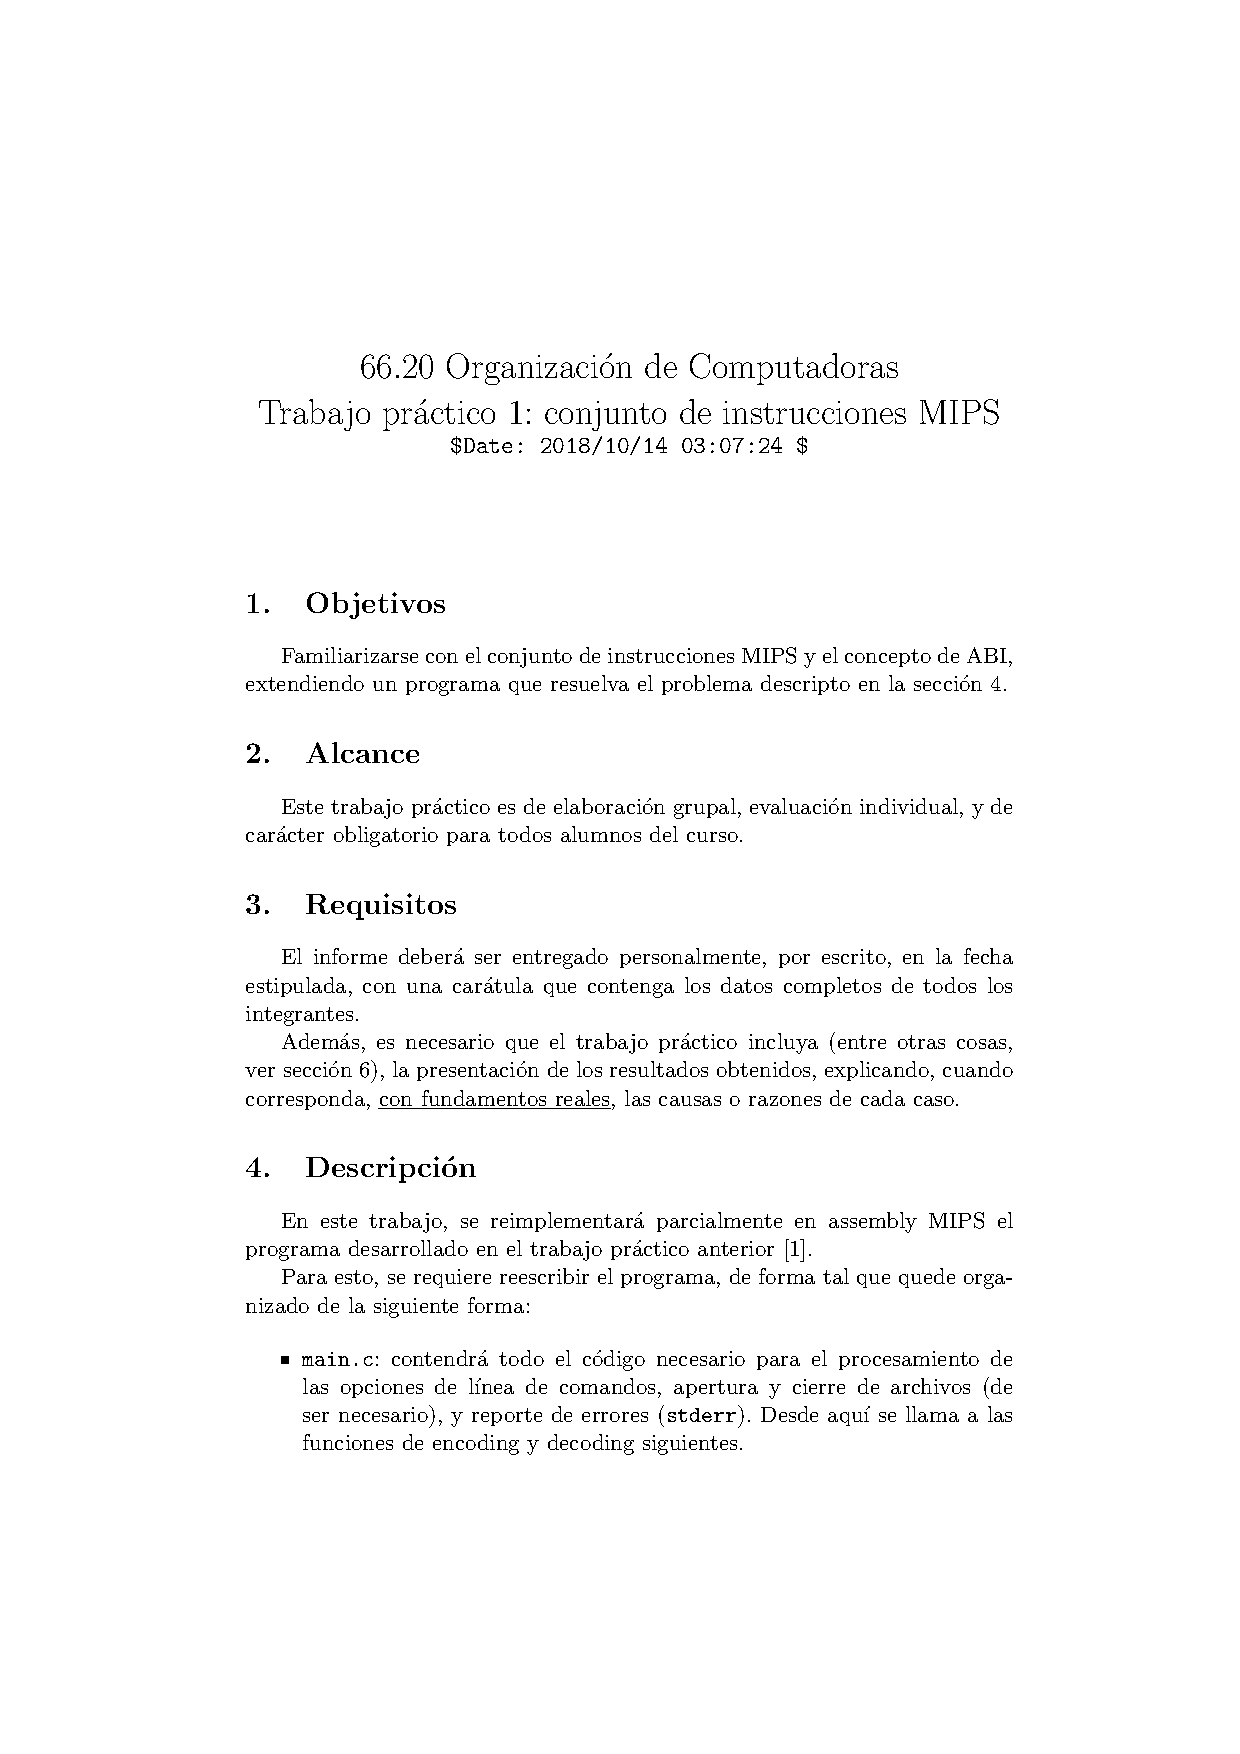
\includepdf[pages=1,scale=0.95,pagecommand = \section{Enunciado del trabajo práctico}\label{enunciado},offset=10 -10]{../tp1-2018-2q.pdf}
\includepdf[pages={2-last},scale=0.95,pagecommand = {},offset=10 -10]{../tp1-2018-2q.pdf}


\newpage

\subsection{Diseño e implementación}

Tomando como referencia el Trabajo Práctico \#0 en donde el programa contenía la lógica tanto del codificador y decodificador y de otras funciones auxiliares, para este nuevo programa, se requirió reescribirlo, de forma tal que quede organizado de la siguiente forma:

\begin{itemize}
	\item{main.c:} contendrá todo el código necesario para el procesamiento de las opciones de línea de comandos, apertura y cierre de archivos (de ser necesario), y reporte de errores (stderr). Desde aquí se llama a las funciones de encoding y decoding siguientes.
	\item {base64.S:} contendrá el cádigo MIPS32 assembly con las funciones base64 encode() y base64 decode(), y las funciones y estructuras de datos auxiliares para realizar los cómputo de encoding y decoding, que
los alumnos crean convenientes. También contendrá la definición en asembly de un vector equivalente al siguiente vector C: const char\* errmsg[]. Dicho vector contendrá los mensajes de error que las funciones antes mencionadas puedan generar, y cuyo índice es el código de error devuelto por las mismas.
	\item{Los header files pertinentes} (al menos, base64.h, con los prototipos de las funciones mencionadas, a incluir en \textit{\textbf{main.c}}), y la declaración del vector extern const char\* errmsg[]).

\end{itemize}

A su vez, las funciones MIPS32 base64 encode() y base64 decode() antes mencionadas, corresponden a los siguientes prototipos C:

	\begin{lstlisting}[language=C]
		int base64 encode(int infd, int outfd)
		int base64 decode(int infd, int outfd)
	\end{lstlisting}

Ambas funciones reciben por \textit{infd} y \textit{outfd} los \textit{file descriptors} correspondientes a los archivos de entrada y salida pre-abiertos por \textit{\textbf{main.c}}, la primera función realizará el encoding a base 64 de su entrada, y la segunda función el decoding de base 64 se su entrada.
Ante un error, ambas funciones volverán con un código de error numérico índice del vector de mensajes de error de \textit{\textbf{base64.h}}), o cero en caso de realizar el procesamiento de forma exitosa.

El programa implementado satisface los siguientes requerimientos, que se detalla a continuación:
\begin{itemize}
	\item{\textbf{ABI}}\\
	 El código presentado utilice la ABI explicada en clase([2] y [3]).
	\item{\textbf{Syscalls}}\\
	Se aclara que desde el código assembly no se llaman funciones que no son escritas originalmente en assembly. Por lo contrario, desde el código C sí se invoca código assembly, particularmente se invocan algunos de los system calls disponibles en NetBSD (en particular, \textit{\textbf{SYSread}} y \textit{\textbf{SYSwrite}}).
\end{itemize}

Como en el Trabajo Práctico \#0, el programa se estructura en los siguientes pasos:
\begin{itemize}
	\item \underline{Análisis de las parámetros de la línea de comandos}: se analizan las opciones ingresadas por la línea de comandos utilizando la función \texttt{getopt\_long()}, la cual puede procesar cada opción que es leída de forma simplificada. Se extraen los argumentos de cada opción y se los guarda dentro de una estructura para su posterior acceso del tipo \texttt{CommandOptions} cuya definición es
	\begin{lstlisting}[language=C]
	typedef struct {
    		File input;
    		File output;
    		const char* input_route;
    		const char* output_route;
    		char error;
    		char encode_opt;
	} CommandOptions;
	\end{lstlisting}
En caso de que no se encuentre alguna opción, se muestra el mensaje de ayuda al usuario para que identifique el prototipo de cómo debe ejecutar el programa.
	
	\item \underline{Validación de opciones:} a medida que se va analizando cada opción de la línea de comandos, se valida cada una de ellas. Si se ingresó algún parámetro no válido para el programa o si se encuentró un error se lo informa al usuario por pantalla y se aborta la ejecución del programa. Se utiliza para ello se la función \texttt{CommandErrArg()} cuyo resultado es:
	\begin{lstlisting}[language=C]
		fprintf(stderr, "Invalid Arguments\n");
    		fprintf(stderr,"Options:\n");
    		fprintf(stderr,"  -V, --version    Print version and quit.\n");
    		fprintf(stderr,"  -h, --help       Print this information.\n");
    		fprintf(stderr,"  -i, --input      Location of the input file.\n");
    		fprintf(stderr,"  -o, --output     Location of the output file.\n");
    		fprintf(stderr,"  -a, --action     Program action: encode (default) or decode.\n");
    		fprintf(stderr,"Examples:\n");
    		fprintf(stderr,"  tp0 -a encode -i ~/input -o ~/output\n");
    		fprintf(stderr,"  tp0 -a decode\n");
	\end{lstlisting}

	Para el caso en que no hubo errores a la validación de los argumentos se procede a llamar a las funciones correspondientes a:
	\begin{itemize}
		\item \texttt{Mensaje de ayuda: } Función \texttt{CommandVersion()}
		\item \texttt{Mensaje de versión: } Función \texttt{CommandHelp()}
		\item \texttt{Input file : } Función \texttt{CommandSetInput()} que guarda la entrada del archivo donde será leído el texto. 
		\item \texttt{Output file: } Función {CommandSetOutput()} que guarda la entrada del archivo de salida donde se escribirá el texto codificado.
		\item \texttt{Acción del programa a ejecutar: } Función {CommandSetEncodeOpt()} que setea la variable $opt->encode\_opt$ indicando si es una operación de ENCODE o DECODE respectivamente.
\end{itemize}

	\item \underline{Encode/Decode:} una vez que se procesó correctamente las opciones de la línea de comandos se procede a llamar a las funciones correspondientes que ejecutarán la operación de ENCODE o DECODE dependiendo del argumento pasado en la línea de comandos. Como se especifico más arriba está parte del programa es implementada en lenguaje assembly MIPS y cumplen lo siguientes:
\begin{itemize}
	\item{DECODE}\\
La operación de DECODE se ejecuta el siguiente código:


	Básicamente lo que se realiza es la lectura del archivo para procesarlo teniendo en cuenta la longitud del archivo a procesar y el padding a decodificar. La función \texttt{Decode()} retorna un buffer de 3 caracteres con el decode de 4 caracteres en base64. Se debe cumplir:\\

 * Pre: el buffer input contiene 4 caracteres. El buffer output tiene por lo menos 3 caracteres
 * Post: retorna un buffer de 3 byte con los caracteres en ASCII. retorna 0 si error 1 si ok.

	\item{ENCODE}\\
La operación de ENCODE se ejecuta el siguiente código:



Básicamente lo que se realiza es la lectura del archivo para procesarlo en la función \texttt{Encode()} en donde recibe 3 caracteres en buffer y los convierte en 4 caracteres codificados en output. Se debe cumplir:\\

 * Pre: el buffer contiene length caracteres (1 a 3) y todos los caracteres son validos
 * Post: retorna un buffer de 4 byte con los caracteres en base64.
	\end{itemize}

	\end{itemize}


\subsection{Parámetros del programa}

Se detallan a continuación los parámetros del programa

\begin{itemize}
    \item -h: Visualiza la ayuda del programa, en la que se indican los parámetros y sus objetivos.
    \item -V: Indica la versión del programa.
    \item -i: Archivo de entrada del programa.
    \item -o: Archivo de salida del programa.
    \item -a: Acción a llevar a cabo: codificación o decodificación.
\end{itemize}

Se indica a continuación detalles respecto a los parámetros:

\begin{itemize}
    \item Si no se explicitan -i y -o, se utilizarán stdin y stdout, respectivamente. 
    \item -V es una opción ``show and quit". Si se explicita este parámetro, sólo se imprimirá la versión, aunque el resto de los parámetros se hayan explicitado. 
    \item -h también es de tipo ``show and quit " y se comporta de forma similar a -V.
    \item en caso de que se use la entrada estándar (con comando echo texto $|$ ./tp0 -a encode) y luego se especifique un archivo de salida con -i, prevalecerá el establecido por parámetro.
\end{itemize}

\subsection{Compilación del programa}

Para obtener un ejecutable, se creó un archivo \texttt{makefile} cuyo contenido es:
	\begin{lstlisting}[language=C]
CC = gcc
CFLAGS = -o0 -g -Wall -Werror -pedantic -std=c99

OBJECTS = command.o encode.o file.c
EXEC = tp0

VALGRIND = valgrind --track-origins=yes --leak-check=full
VALGRIND-V = $(VALGRIND) -v

all: $(EXEC)

command.o: command.c command.h
	$(CC) $(CFLAGS) -c command.c -o command.o
encode.o: encode.c encode.h
	$(CC) $(CFLAGS) -c encode.c -o encode.o
file.o: file.c file.h
	$(CC) $(CFLAGS) -c file.c -o file.o

$(EXEC): $(OBJECTS)
	$(CC) $(CFLAGS) $(OBJECTS) main.c -o $(EXEC) -lm

run: $(EXEC)
	./$(EXEC)

valgrind: $(EXEC)
	$(VALGRIND) ./$(EXEC)

valgrind-verb: $(EXEC)
	$(VALGRIND-V) ./$(EXEC)

clean:
	rm -f *.o $(EXEC)
	\end{lstlisting}


Para ejecutarlo, posicionarse en el directorio \texttt{src/} y ejecutar el siguiente comando:
\begin{lstlisting}
$ make
\end{lstlisting}

Para proceder a la ejecución del programa, se debe llamar a:

\begin{lstlisting}
$ ./tp0
\end{lstlisting}

seguido de los parámetros que se desee modificar, los cuales se indicaron en la sección 1.2.

En caso de ser entrada estándar (stdin) se podrá ejecutar de la siguiente forma:

\begin{lstlisting}
$ echo texto | ./tp0 -a encode
\end{lstlisting}

También en este caso, se indican a continuación los parámetros a usar.

Para el caso de hacerlo en el emulador GXemul que provee la cátedra, utilizando la máquina virtual que contiene el sistema operativo NetBSD, no se utilizó el archivo Makefile, la compilación se realizó con la herramienta \texttt{gcc}.
\newpage


\section{Pruebas realizadas}


\subsection{Pruebas con archivo bash test-automatic.sh}
Para la ejecución del siguiente script se debe copiar, se debe ubicar el archivo ejecutable compilado dentro de la carpeta de test para que se ejecuten correctamente las pruebas. El script sería:

\begin{lstlisting}
#!/bin/bash

echo "#########################################"
echo "########## Tests automaticos  ###########"
echo "#########################################"

mkdir ./outputs

echo "#---------# COMIENZA test ejercicio 0 archivo vacio #--------#"
touch ./outputs-aut/zero.txt
./tp1 -a encode -i ./outputs-aut/zero.txt -o ./outputs-aut/zero.txt.b64
ls -l ./outputs-aut/zero.txt.b64

if diff -b ./outputs-aut/zero.txt ./outputs-aut/zero_ok.txt; then
 echo "[OK]";
else echo ERROR;
fi

echo "#---------# FIN test ejercicio 0 archivo vacio #--------#"
echo "#-------------------------------------------------------#"
echo "#---------# COMIENZA test ejercicio 1 archivo vacio sin -a #--------#"

touch ./outputs-aut/zero.txt
./tp1 -i ./outputs-aut/zero.txt -o ./outputs-aut/zero.txt.b64
ls -l ./outputs-aut/zero.txt.b64

if diff -b ./outputs-aut/zero.txt ./outputs-aut/zero_ok.txt; then
 echo "[OK]";
else echo ERROR;
fi

echo "#---------# FIN test ejercicio 1 archivo vacio sin -a #--------#"
echo "#--------------------------------------------------------------#"
echo "#---------# COMIENZA test ejercicio 2 stdin y stdout #---------#"

echo -n Man | ./tp1 -a encode > ./outputs/outputEncode.txt
if diff -b ./outputs-aut/outputEncode-aut.txt ./outputs/outputEncode.txt; then echo "[OK]"; else
	echo ERROR;
fi

echo "#---------# FIN test ejercicio 2 stdin y stdout #--------#"
echo "#--------------------------------------------------------#"
echo "#---------# COMIENZA test ejercicio 3 stdin y stdout #--------#"

echo -n TWFu | ./tp1 -a decode > ./outputs/outputDecode.txt
if diff -b ./outputs-aut/outputDecode-aut.txt ./outputs/outputDecode.txt; then echo "[OK]"; else
	echo ERROR;
fi

echo "#---------# FIN test ejercicio 3 stdin y stdout #--------#"
echo "#--------------------------------------------------------#"
echo "#---------# COMIENZA test ejercicio 3 help sin parámetros #--------#"

./tp1 > ./outputs/outputMenuHelp.txt
if diff -b ./outputs-aut/outputMenuHelp-aut.txt ./outputs/outputMenuH.txt; then echo "[OK]"; else
	echo ERROR;
fi

echo "#---------# FIN test ejercicio 3 help sin parámetros #--------#"
echo "#-----------------------------------------------------#"
echo "#----------# COMIENZA test menu help (-h) #----------#"

./tp1 -h > ./outputs/outputMenuH.txt

if diff -b ./outputs-aut/outputMenuHelp-aut.txt ./outputs/outputMenuH.txt; then echo "[OK]"; else
	echo ERROR;
fi

echo "#----------# FIN test menu version (-h) #----------#"
echo "#-----------------------------------------------------#"
echo "#----------# COMIENZA test menu help (--help) #----------#"

./tp1 --help > ./outputs/outputMenuHelp.txt

if diff -b ./outputs-aut/outputMenuHelp-aut.txt ./outputs/outputMenuHelp.txt; then echo "[OK]"; else
		echo ERROR;
fi

echo "#----------# FIN test menu version (--help) #----------#"
echo "#-----------------------------------------------------#"
echo "#----------# COMIENZA test menu version (-V) #----------#"

./tp1 -V > ./outputs/outputMenuV.txt

if diff -b ./outputs-aut/outputMenuVersion-aut.txt ./outputs/outputMenuV.txt; then echo "[OK]"; else
		echo ERROR;
fi
echo "#----------# FIN test menu version (-V) #----------#"
echo "#-----------------------------------------------------#"
echo "#----------# COMIENZA test menu version (--version) #----------#"

./tp1 --version > ./outputs/outputMenuVersion.txt

if diff -b ./outputs-aut/outputMenuVersion-aut.txt ./outputs/outputMenuVersion.txt; then echo "[OK]"; else
		echo ERROR;
fi
echo "#----------# FIN test menu version (--version) #----------#"
echo "#-----------------------------------------------------#"
echo "#---------# COMIENZA test ejercicio encode/decode #--------#"

echo xyz | ./tp1 -a encode | ./tp1 -a decode | od -t c

echo "#---------# FIN test ejercicio encode #--------#"
echo "#-----------------------------------------------------#"
echo "#---------# COMIENZA test ejercicio longitud maxima 76 #--------#"

yes | head -c 1024 | ./tp1 -a encode > ./outputs/outputSize76.txt

if diff -b ./outputs-aut/outputSize76-aut.txt ./outputs/outputSize76.txt; then echo "[OK]"; else
		echo ERROR;
fi

echo "#---------# FIN test ejercicio longitud maxima 76 #--------#"
echo "#-----------------------------------------------------#"
echo "#---------# COMIENZA test ejercicio decode 1024 #--------#"

yes | head -c 1024 | ./tp1 -a encode | ./tp1 -a decode | wc -c > ./outputs/outputSize1024.txt

if diff -b ./outputs-aut/outputSize1024-aut.txt ./outputs/outputSize1024.txt; then echo "[OK]"; else
		echo ERROR;
fi

echo "#---------# FIN test ejercicio decode 1024#--------#"
echo "#-----------------------------------------------------#"
echo "#---------# COMIENZA test ejercicio encode/decode random #--------#"

n=1;
while :; do
#while [$n -lt 10]; do
head -c $n </dev/urandom >/tmp/in.bin;
./tp1 -a encode -i /tmp/in.bin -o /tmp/out.b64;
./tp1 -a decode -i /tmp/out.b64 -o /tmp/out.bin;
if diff /tmp/in.bin /tmp/out.bin; then :; else
echo ERROR: $n;
break;
fi
echo [OK]: $n;
n=`expr $n + 1`;
rm -f /tmp/in.bin /tmp/out.b64 /tmp/out.bin
done

echo "#---------# FIN test ejercicio encode/decode random #--------#"
echo "#------------------------------------------------------------#"

echo "##########################################"
echo "####### FIN Tests automaticos  ###########"
echo "##########################################"
\end{lstlisting}

El cual no presenta errores en ninguna de las corridas llevadas a cabo.


Todas las pruebas que se presentan a continuación, están codificadas en los archivos de prueba ***.txt de forma que puedan ejecutarse y comprobar los resultados obtenidos.

Se indicaran a continuación lo siguiente: comandos para ejecutarlas, líneas de código que las componen y resultado esperado.


\subsubsection{Generales}


\begin{itemize}
    \item Mensaje de ayuda\\
    
\begin{lstlisting}
$ ./tp0 -h  o ./tp0 --help

Options:
  -V, --version    Print version and quit.
  -h, --help       Print this information.
  -i, --input      Location of the input file.
  -o, --output     Location of the output file.
  -a, --action     Program action: encode (default) or decode.
Examples:
  tp0 -a encode -i ~/input -o ~/output
  tp0 -a decode


\end{lstlisting}     
     
	\item Mensaje de version\\

            \begin{lstlisting}
$ ./tp0 -V  o ./tp0 --version
Version: 0.1
             \end{lstlisting}  
         
         
    \item Archivo de entrada no válido
            \begin{lstlisting}
$ ./tp0 -i archivoInvalido.txt

Invalid Arguments
Options:
  -V, --version    Print version and quit.
  -h, --help       Print this information.
  -i, --input      Location of the input file.
  -o, --output     Location of the output file.
  -a, --action     Program action: encode (default) or decode.
Examples:
  tp0 -a encode -i ~/input -o ~/output
  tp0 -a decode


             \end{lstlisting}  

\end{itemize}


\newpage

\section{Conclusiones}

El trabajo práctico nos permitió desarrollar una API para procesar archivos transformándolos a su equivalente \texttt{base64} en lenguaje C y, en parte, en lenguaje assembly MIPS para la codificación y decodificación de los archivos. Además, nos permitió familiarizarnos con las \texttt{syscalls} para el llamado de las funciones en lenguaje assembly y el consecuente análisis y desarrollo de código assembler MIPS utilizando el emulador GXemul.


\begin{thebibliography}{10}
	\bibitem{}Enunciado del primer trabajo práctico (TP0), primer cuatrimestre de 2018.
	\bibitem{}Base64 (Wikipedia) http://en.wikipedia.org/wiki/Base64
	\bibitem{}The NetBSD project, http://www.netbsd.org/
	\bibitem{book_Cprogr} Kernighan, B. W. - Ritchie, D. M. - \emph{C Programming Language} - 2\textsuperscript{nd} edition - Prentice Hall - 1988.
	\bibitem{gnu_make} \emph{GNU Make} - \hyperlink{make}{https://www.gnu.org/software/make/}
	\bibitem{valgrind} \emph{Valgrind} - \hyperlink{valgrind}{http://valgrind.org/}
	\bibitem{}MIPS ABI: Function Calling, Convention Organización de computadoras(66.20) en archivo ''func\ call\ conv.pdf'' y enlace http://groups.yahoo.com/groups/orga-comp/Material/)
	\bibitem{}System V application binary interface, MIPS RISC processor supplement
(third edition). Santa Cruz Operations, Inc.
\end{thebibliography}
\newpage
%-----------------------------------%
%									%
%			Seccion:Fuente			%
%									%
%-----------------------------------%
\appendix
\section{Código fuente}\label{appendix_codigo_fuente}

\subsubsection{main.c}\label{main}
\lstinputlisting[language=C]{../src/main.c}

\newpage

\subsubsection{Assembly base64.S}\label{base64.S}
\lstinputlisting[style=customasm]{../src/base64.S}

\newpage

\subsubsection{Header file base64.h}\label{base64.h}
\lstinputlisting[language=C]{../src/base64.h}


\end{document}
